% This file was created with tikzplotlib v0.10.1.
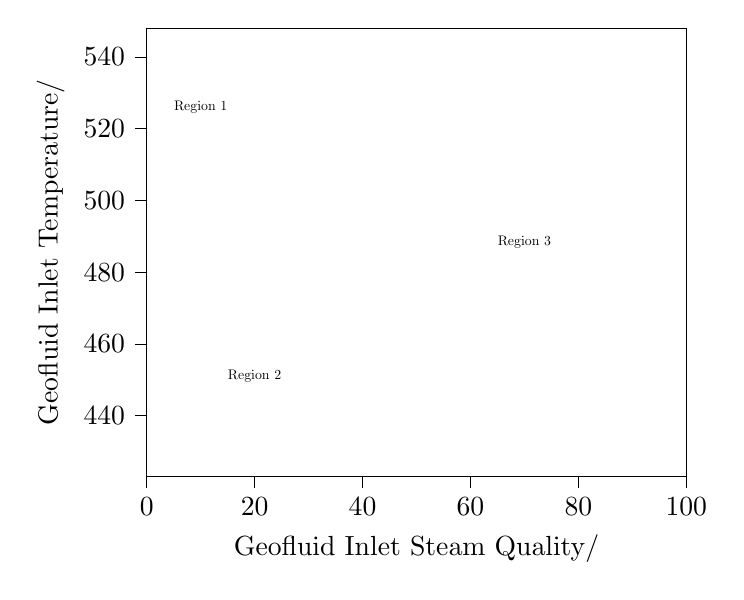
\begin{tikzpicture}

\definecolor{darkgray176}{RGB}{176,176,176}
\definecolor{lightgray204}{RGB}{204,204,204}

\begin{axis}[
legend style={fill opacity=0.8, draw opacity=1, text opacity=1, draw=lightgray204},
tick align=outside,
tick pos=left,
x grid style={darkgray176},
xlabel={Geofluid Inlet Steam Quality/\unit{\percent}},
xmin=0, xmax=100,
xtick style={color=black},
y grid style={darkgray176},
ylabel={Geofluid Inlet Temperature/\unit{\K}},
ymin=423, ymax=548,
ytick style={color=black}
]
\draw (axis cs:70,487.5) node[
  scale=0.5,
  anchor=base,
  text=black,
  rotate=0.0
]{Region 3};
\draw (axis cs:20,450) node[
  scale=0.5,
  anchor=base,
  text=black,
  rotate=0.0
]{Region 2};
\draw (axis cs:10,525) node[
  scale=0.5,
  anchor=base,
  text=black,
  rotate=0.0
]{Region 1};
\end{axis}

\end{tikzpicture}
